\section{Fase 5: Refactor del proyecto y consolidación del generador}
\label{sec:refactor-consolidacion-generador}

Una vez realizadas las primeras pruebas y añadidas muchas trazas para comprobar los diferentes errores surgidos en el proceso de generacion, el codigo del 
fichero \textbf{project\_generator.py} habia crecido demasiado y se habia convertido en un fichero dificil de depurar, y aprovechando este momento de refactorizacion se realizaron mas cambios sobre gran parte de codigos del proyecto.

Esta fase se divido en dos partes importantes. En primer lugar a la refactorizacion de partes importantes, como el fichero comentado anteriormente de mucho ficheros html y css, haciendo su uso y modificacion futura mucho mas sencilla al tener todo divido en modulos.

\subsection{Refactor del generador en modulos}
\label{subsec:refactor-generador-modulos}

Estos cambios fueron muy importantes, los pasos del generador se realizaban con 
todo el contenido dentro del mismo fichero, algo que no era de facil escalabilidad 
a futuro, por lo que el primer cambio fue dividir el \textbf{project\_generator.py} 
en cuatro ficheros encargados cada uno de una labor especifica dentro de 
\textbf{utils/generator}, como se muestra en la Figura~\ref{fig:modulos-generador}.

\begin{figure}[H]
    \centering
    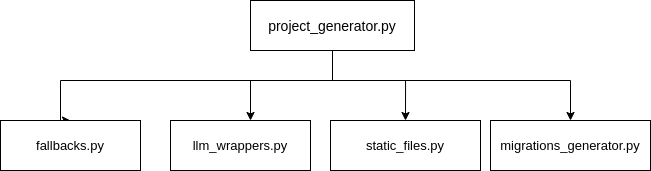
\includegraphics[width=0.8\textwidth]{img/disenoimplementacion/modulosgenerador}
    \caption{Estructura de módulos del generador tras el refactor}
    \label{fig:modulos-generador}
\end{figure}

\begin{itemize}
    \item \textbf{\texttt{llm\_wrappers.py}}: Centralizó todas las llamadas al LLM en tres funciones reutilizables. \texttt{llm\_call} para llamadas básicas que devuelven texto, \texttt{llm\_json\_call} para llamadas que esperan JSON como respuesta, y \texttt{llm\_call\_logged} para llamadas que además guardan un registro en base de datos para mejorar la depuracion. Esta ultima funcion fue muy importante en el proceso de generacion y depuracion, anteriormente si algo fallaba no habia forma de saber que habia pasado, pero de esta forma cada vez que se llamaba al LLM durante la generación de un proyecto, además de hacer la llamada normal, guardaba automáticamente en base de datos un registro con toda la información de esa llamada: el paso que se estaba generando, el prompt enviado, la respuesta recibida y si había habido algún error. Ese registro se guarda en \texttt{GenerationLog}
    
    \item \textbf{\texttt{fallbacks.py}}: Agrupó todos los fallbacks de emergencia en un único fichero. Cada función de este módulo generaba una versión mínima pero funcional de un artefacto concreto del proyecto: páginas, modelos, vistas o templates. Al tenerlos centralizados resultaba mucho más sencillo mejorarlos o ajustarlos sin tocar el orquestador principal.
    
    \item \textbf{\texttt{static\_files.py}}: Extrajo toda la generación de ficheros de infraestructura que no dependen del LLM: \texttt{manage.py}, \texttt{settings.py}, \texttt{wsgi.py}, \texttt{urls.py}, \texttt{Dockerfile}, \texttt{entrypoint.sh} y \texttt{requirements.txt}. El orquestador principal quedó así mucho más limpio, delegando en este módulo la construcción del scaffolding fijo.
    
    \item \textbf{\texttt{migrations\_generator.py}}: Aisló la lógica de generación automática de la migración inicial, que parseaba el \texttt{models.py} producido por el LLM y construía el fichero \texttt{0001\_initial.py} correspondiente.
\end{itemize}


\subsection{Refactor de templates y ficheros de estilos}
\label{subsec:refactor-templates-estilos}

La misma causa que creo la decision del refactor del generador ocurrio con los ficheros de presentacion del proyecto (HTML, CSS y JavaScript).
Hasta el momento los templates HTML eran ficheros que incluian todas las secciones en un unico bloque, al igual que ocurria con los ficheros CSS y JavaScript. Como comentaba anteriormente, esta fase introdujo una reorganizacion completa de la interfaz con la separacion de responsabilidades.

En cuanto a los templates se creo un nuevo modulo \textbf{partials}, encargado de contener los fragmentos que representan una seccion concreta de cada pagina. Cada fichero principal paso a contener sus partials, incluyendose mediante la etiqueta \textbf{include} de Django.

La home del proyecto, que hasta entonces era el fichero mas complejo, se dividió en seis partials independientes dentro de \texttt{templates/WebBuilder/partials/home}, quedando asi la nueva estructura:

\begin{itemize}
    \item \texttt{hero.html} — la sección principal de bienvenida
    \item \texttt{examples.html} — ejemplos de sitios generados
    \item \texttt{how.html} — explicación del funcionamiento
    \item \texttt{llms.html} — sección de modelos de lenguaje compatibles
    \item \texttt{metrics.html} — métricas públicas del sistema
    \item \texttt{cta.html} — botón de acceso a la aplicación
\end{itemize}

El asistente se dividió en tres partials dentro de \texttt{templates/WebBuilder/partials/assistant/}:

\begin{itemize}
    \item \texttt{input.html} — formulario del paso 1, donde el usuario 
    introduce la URL de la API o sube un fichero local para su análisis
    \item \texttt{analysis.html} — resultado del paso 2, que muestra las 
    estadísticas del dataset analizado: número de items encontrados, campos 
    disponibles y ruta de la colección principal
    \item \texttt{preview.html} — resultado del paso 3, donde se muestra 
    el schema propuesto por la IA y el usuario puede revisarlo y aprobarlo 
    antes de continuar
\end{itemize}

El historial se dividió en dos partials dentro de \texttt{templates/WebBuilder/partials/history/}:

\begin{itemize}
    \item \texttt{published\_sites.html} — listado de sitios ya generados 
    y desplegados por el usuario
    \item \texttt{recent\_analysis.html} — listado de análisis recientes 
    realizados por el usuario
\end{itemize}

Los ficheros estáticos sufrieron una reorganización equivalente. 
El CSS pasó a estar organizado por página y por sección dentro de 
\texttt{static/css/}:

\begin{itemize}
    \item \texttt{home/hero.css} — estilos de la sección principal de bienvenida
    \item \texttt{home/examples.css} — estilos de la sección de ejemplos
    \item \texttt{home/how.css} — estilos de la sección de funcionamiento
    \item \texttt{home/llms.css} — estilos de la sección de modelos compatibles
    \item \texttt{home/metrics.css} — estilos de la sección de métricas públicas
    \item \texttt{home/cta.css} — estilos de la sección de acceso a la aplicación
    \item \texttt{assistant.css} — estilos del asistente de generación
    \item \texttt{history.css} — estilos del historial del usuario
    \item \texttt{edit.css} — estilos de la página de edición del schema
    \item \texttt{login.css} — estilos de las páginas de login y registro
    \item \texttt{navbar.css} — estilos de la barra de navegación
    \item \texttt{backgrounds.css} — fondos y efectos visuales compartidos
\end{itemize}

El JavaScript siguió el mismo criterio con ficheros independientes 
por página en \texttt{static/js/}:

\begin{itemize}
    \item \texttt{home.js} — lógica interactiva de la home
    \item \texttt{assistant.js} — lógica del flujo del asistente
    \item \texttt{edit.js} — lógica de la edición del schema
    \item \texttt{site\_render.js} — lógica de la vista previa del sitio generado
\end{itemize}

El \texttt{base.html} se actualizó para cargar las fuentes de Google Fonts 
necesarias para el nuevo diseño: Inter para el texto general, 
y Geist y Geist Mono para elementos de código y datos técnicos.

Esta reorganización, aunque invisible para el usuario final, facilitó enormemente el mantenimiento y la evolución de la interfaz en los sprints siguientes, ya que cualquier cambio en una sección concreta de una página solo requería tocar un fichero pequeño y bien delimitado.


\subsection{Enriquecimiento de prompts}
\label{subsec:enriquecimiento-prompts}

Tras unas cuantas pruebas, llegue a la conclusion de un problema importante, podria ocurrir que un usuario no familiarizado con los prompts de IA no supiese como hacerlo adecuadamente, o que incluso lo dejase vacio. Para resolver este problema se creo el fichero \texttt{utils/llm/enrich\_prompts.py}, 
encargado de analizar automaticamente los campos del dataset antes de construir el prompt y añadir contenido personalizado.
Si el dataset tenia campos con imagenes se le indica al modelo que las usara de forma destacada. Si tenia precios, que los resalte visualmente. Si tenia
fechas que las mostrara de forma clara. De esta forma se garantiza que el LLM siempre recibiera suficiente contexto para tomar decisiones razonadas.
De todos modos si algo no estuviese en la mente del usuario, en el siguiente paso de editar el schema podria modificarlo añadiendo los campos necesarios o modificando los existentes.


\subsection{Trazabilidad: GenerationLog}
\label{subsec:trazabilidad-generationlog}

Anteriormente en las generaciones si algo fallaba no había forma de saber qué prompt se había enviado exactamente, qué había respondido el modelo ni si había habido reintentos. Para arreglar esto se creo el modelo \textbf{GenerationLog}, vinculado mediante una clave a su correspondiente \textbf{GeneratedSite}. 

Cada llamada al LLM durante la generación de un proyecto producía un registro que almacenaba el paso concreto que se estaba generando, el modelo de LLM utilizado, el prompt de sistema y el prompt de usuario enviados, la respuesta en crudo devuelta por el modelo, los errores de consistencia detectados y si la llamada había necesitado un reintento. Esto permitía analizar a posteriori qué pasos fallaban con más frecuencia, qué modelos producían mejores resultados y qué tipos de datasets generaban más inconsistencias.


\subsection{Verificacion de consistencia}
\label{subsec:verificacion-consistencia}

Otro problema frecuente era que el LLM no tenia suficiente contexto entre ficheros, principal causa de las alucinaciones del LLM. Ocurria lo siguiente:
se definia un campo con un nombre en \textbf{models.py} y luego en los demas ficheros se referenciaba con ligeros cambios, provocando errores de ejecución.
Para detectar estos casos antes de que el usuario desplegase el proyecto, se implemento el fichero \texttt{utils/llm/consistency\_checker.py}.

Este fichero extraía mediante expresiones regulares los campos definidos en \texttt{models.py} y buscaba en los demas templates las referencias a esos campos. Cualquier referencia encontrada diferente que no correspondiera al campo real del modelo, se registraba como error de consistencia. 
Estos errores se guardaban en el campo \texttt{consistency\_errors} del modelo \texttt{GenerationLog} correspondiente, permitiendo identificar que pasos producian mas inconsistencias y como se producian, para el consiguiente arreglo a futuro.


\subsection{Panel de métricas}
\label{subsec:panel-metricas}

Para tener un uso mas sencillo y accesible del contenido de GenerationLog añadi una vista de metricas en \textbf{views/metrics.py}, accesible unicamente para usuarios con permisos de administrador. El objetivo de esta vista era tener visibilidad real sobre el comportamiento del generador, los fallos mas recurrentes, que modelos eran mas optimos para cada tipo de pagina, etc.

El panel mostraba las siguientes estadísticas agregadas:

\begin{itemize}
    \item \textbf{Resumen general}: número total de registros en \texttt{GenerationLog}, sitios generados y análisis realizados hasta la fecha.
    \item \textbf{Desglose por paso}: para cada uno de los siete pasos del generador, se mostraba el número de llamadas realizadas, cuántas habían necesitado reintento y la tasa de reintento resultante. Esto permitía identificar qué pasos eran más problemáticos y priorizar las mejoras.
    \item \textbf{Distribución por modelo}: agrupación de las llamadas por modelo de LLM utilizado, lo que facilitaba comparar el rendimiento de distintos proveedores cuando se probaban configuraciones diferentes.
\end{itemize}

Esta informacion resulto util para mejorar las siguientes fases donde cambios minimos producirian grandes resultados.


